%% CAPITULO 3 -- PROCEDIMENTOS METODOLOGICOS

\section{Procedimentos metodológicos}

Esta pesquisa é aplicada e exploratória, com abordagem qualitativa. Nesta versão, o procedimento previsto é uma revisão bibliográfica estruturada sobre a triagem de manifestações com inteligência artificial, seguida da comparação do contexto institucional e da tarefa tratada em cada estudo.

As buscas previstas utilizam bases abertas de metadados bibliográficos, com termos em português, inglês e espanhol e registro da data, da fonte e da expressão de busca. Os estudos selecionados são lidos ao menos pelo resumo, e os achados só são atribuídos ao que o conteúdo efetivamente consultado sustenta.

A Figura~\ref{fig:fluxo-triagem} apresenta o fluxo genérico de triagem que orienta a análise, desde o recebimento da manifestação até a revisão humana da proposta de encaminhamento.

\begin{figure}[htb]
  \caption{Fluxo genérico de triagem de manifestações com supervisão humana}
  \label{fig:fluxo-triagem}
  \centering
  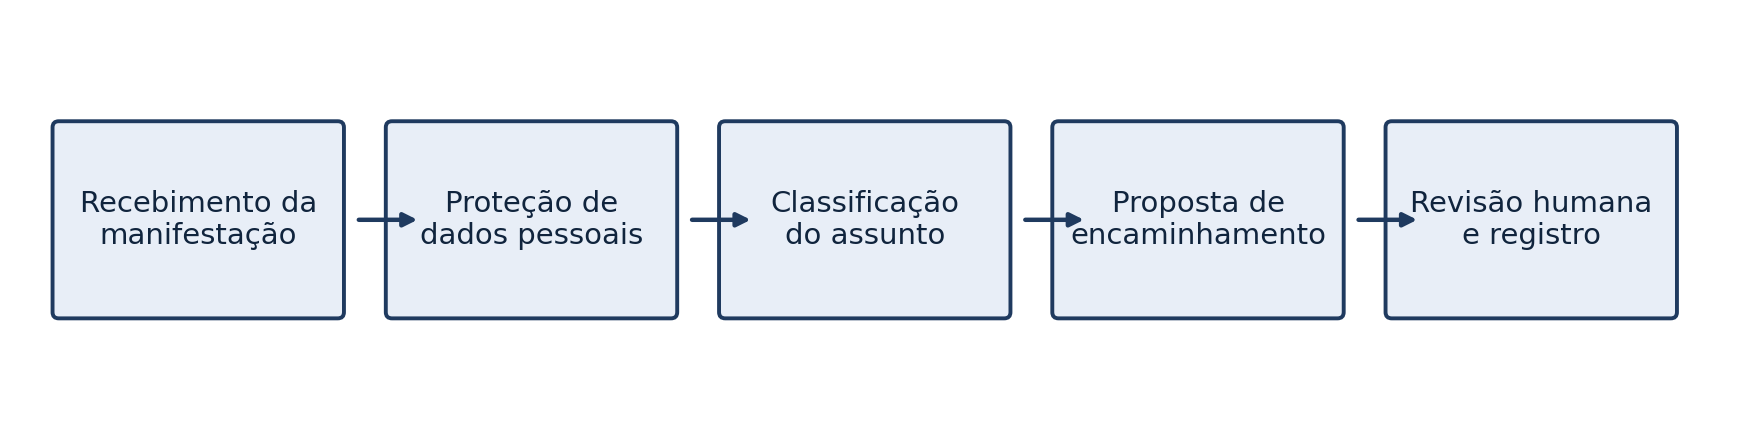
\includegraphics[width=0.95\textwidth]{figuras/fluxo-triagem.png}
  \fonte{Elaboração própria.}
\end{figure}
